%; whizzy paragraph -pdf xpdf -latex ./whizzypdfptex.sh
%; whizzy-paragraph "^\\\\begin{frame}"
% latex beamer presentation.
% platex, latex-beamer でコンパイルすることを想定。 

%     Tokyo Debian Meeting resources
%     Copyright (C) 2009 Junichi Uekawa
%     Copyright (C) 2009 Nobuhiro Iwamatsu

%     This program is free software; you can redistribute it and/or modify
%     it under the terms of the GNU General Public License as published by
%     the Free Software Foundation; either version 2 of the License, or
%     (at your option) any later version.

%     This program is distributed in the hope that it will be useful,
%     but WITHOUT ANY WARRANTY; without even the implied warreanty of
%     MERCHANTABILITY or FITNESS FOR A PARTICULAR PURPOSE.  See the
%     GNU General Public License for more details.

%     You should have received a copy of the GNU General Public License
%     along with this program; if not, write to the Free Software
%     Foundation, Inc., 51 Franklin St, Fifth Floor, Boston, MA  02110-1301 USA

\documentclass[cjk,dvipdfmx,12pt]{beamer}
\usetheme{Tokyo}
\usepackage{monthlypresentation}

%  preview (shell-command (concat "evince " (replace-regexp-in-string "tex$" "pdf"(buffer-file-name)) "&")) 
%  presentation (shell-command (concat "xpdf -fullscreen " (replace-regexp-in-string "tex$" "pdf"(buffer-file-name)) "&"))
%  presentation (shell-command (concat "evince " (replace-regexp-in-string "tex$" "pdf"(buffer-file-name)) "&"))

%http://www.naney.org/diki/dk/hyperref.html
%日本語EUC系環境の時
\AtBeginDvi{\special{pdf:tounicode EUC-UCS2}}
%シフトJIS系環境の時
%\AtBeginDvi{\special{pdf:tounicode 90ms-RKSJ-UCS2}}

\title{OSC 2011 Tokyo/Fall \\東京エリアDebian勉強会}
\subtitle{第82回 2011年11月度}
\author{岩松 信洋 iwamatsu@debian.org\\IRC nick: iwamatsu}
\date{2011年11月19日}
\logo{
\includegraphics[width=8cm]{image200607/openlogo-light.eps}}

\begin{document}

\frame{\titlepage{}}

%\section{}

\begin{frame}{Agenda}
 \begin{itemize}
  \item Debian勉強会とは?
  \item Debian topic update / 3月からのアップデート内容
  \item Debian topic update / Whezzyに向けての作業
  \item 質疑応答
 \end{itemize}
\end{frame}

\begin{frame}{自己紹介}
\begin{itemize}
\item 岩松信洋 (Nobuhiro Iwamatsu)
\item Twitter: @iwamatsu
\item Debian Project Official Developer
\item bluetooth 全般、libpng, OpenCV, 組込関係、Renesas SH ポート etc..
\item Linux kernel 開発、U-Boot 開発、etc...
\end{itemize}
\end{frame}

\emtext{Debian 勉強会とは?}

\begin{frame}{Debian 勉強会とは?}
\begin{itemize}
\item Debian ユーザとDebian開発者がフェイス・トゥ・フェイスで話し合う場
\item Debian 開発者および開発者予備軍を育成する場
\item Debianの最新情報、バッドノウハウを提供する場
\item 東京(関東)と関西で月に一回開催\\
\url{http://tokyodebian.alioth.debian.org/}
\item Debian Hack Cafe\\
毎月平日、何処かのカフェで雑談しながら Debian を開発しています。\\
@debian\_hackcafe でアナウンスされます。\\
\item お気軽にご参加ください。
\end{itemize}
\end{frame}

\emtext{Debian topic update\\3月からのアップデート内容}

\begin{frame}
\begin{center}
\LARGE{OSC2011 Tokyo/Spring(3月)からの更新を見てみましょう。}
\end{center}
\end{frame}

\begin{frame}
 \frametitle{Debian topic update}
\begin{center}
\LARGE{Squeeze がリリースされてから約9ヶ月経ったわけですが......}\\\pause
\LARGE{3回アップデートされていますよ!}
\end{center}
\end{frame}

\begin{frame}
 \frametitle{Debian topic update / squeeze update}
\begin{itemize}[<+->]

\item 2011/03/19 Debian 6.0.1 released\\
27個のセキュリティ修正と、68個のパッケージを更新。\\
インストーラーの改善(armelのNASサポート、iBook(ppc), Cobalt(mips))

\item 2011/06/25 Debian 6.0.2 released\\
59個のセキュリティ修正と、73個のパッケージを更新

\item 2011/10/08 Debian 6.0.3 released\\
52個のセキュリティ修正と、83個のパッケージを更新\\
いくつかのGiga-bit Ether をサポート (tg3, e1000e, igb, r8169)\\

\end{itemize}

%\pause
%\small{\url{http://ftp.debian.org/debian/dists/squeeze/ChangeLog}}\\

\end{frame}

\begin{frame}
\begin{center}
\LARGE{lennyもアップデートされていますよ!}
\end{center}
\end{frame}

\begin{frame}
 \frametitle{Debian topic update / lenny update}
\begin{itemize}

\item 2011/10/01 Debian 5.0.9 released\\
90個のセキュリティ修正と、18個のパッケージを更新

\end{itemize}
\end{frame}

\begin{frame}
\begin{center}
\LARGE{アップデートしてない人は 今すぐ apt-get update \&\& apt-get upgrade!}
\end{center}
\end{frame}

\begin{frame}
\begin{center}
\LARGE{パッケージ数}
\end{center}
\end{frame}

\begin{frame}{パッケージ数}
\begin{itemize}[<+->]

%\item 2011年3月
%\item 2011年11月

\item squeeze(stable)\\
バイナリパッケージ数: 28130\\
ソースパッケージ数  : 14609

\item whezzy(testing)\\ 
バイナリパッケージ数: 33274 {\color{red}+5144}\\
ソースパッケージ数  : 16333 {\color{red}+1724}

\item sid(unstable)\\ 
バイナリパッケージ数: 34852 {\color{red}+1578}\\
ソースパッケージ数  : 17376 {\color{red}+1043}
\end{itemize}

\end{frame}

\begin{frame}
\begin{center}
\LARGE{バグの数}
\end{center}
\end{frame}


\begin{frame}{バグの総数}
\begin{itemize}[<+->]
\item 2011年03月: 約616000
\item 2011年11月: 約649100
\item 約9ヶ月で約33000のバグレポート。
\item 閉じられたバグ: 約30000。
\end{itemize}

\end{frame}

\begin{frame}
\begin{center}
\LARGE{開発者数}
\end{center}
\end{frame}


\begin{frame}{開発者数}
\begin{itemize}[<+->]
\item 2011年03月\\
Debian Develope 約1440名 \\
Debian Maintainer 約80名

\item 2011年11月\\
Debian Develope 約1470名 \\
Debian Maintainer 約80名

\item 57ヶ国\\
日本人は 46名(アクティブメンバは33名)

\end{itemize}
\end{frame}

\begin{frame}
\begin{center}
\LARGE{Debian カンファレンス}
\end{center}
\end{frame}

\begin{frame}{Debconf / Debian カンファレンス}
\begin{itemize}
\item 今年のDebconf, Debconf11 はボスニアヘルツェゴビナ
参加者は約400名。日本からは3名参加。

\item 来年のDebconf, Debconf12 はニカラグアで開催。\\
2012年7月8日 から 14日 まで。
\end{itemize}
\end{frame}


\begin{frame}
\begin{center}
\LARGE{新たに開始された\\サービス/プロジェクト}
\end{center}
\end{frame}


\begin{frame}{新たに開始されたサービス/プロジェクト}
\begin{itemize}[<+->]
\item Debian Derivatives Exchange\\
Debianと派生したディストリビューションの技術的を共有するためのプロジェクト。\\
実はDebian、派生されているディストリビューション1位。
\item CUT(2 Usable Testing) プロジェクト\\
rolling 思考のディストリビューションのサポート
\item Emdebian による Emdebian Grip の Debian への統合
\end{itemize}
\end{frame}


\begin{frame}
 \frametitle{Debian topic update / Linux 20歳}
\begin{center}

\Large{Linux 20歳。}\\

\includegraphics[width=0.5\hsize]{image201111/linux_20_years_082511.jpg}
\end{center}
\end{frame}
% cakeの画像は以下からダウンロード
% http://www.ecualug.org/2006/08/16/galerias_de_imagenes/debian_cake


\begin{frame}
 \frametitle{Debian topic update / Debian 18歳}
\begin{center}

\Large{2011年8月16日。Debian 18歳。}\\
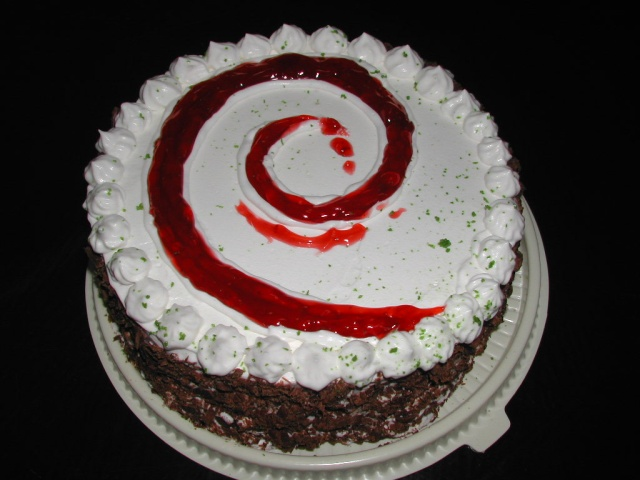
\includegraphics[width=0.8\hsize]{image201111/debian-cake.jpg}
\end{center}
\end{frame}
% 画像は以下からダウンロード
% http://techgage.com/images/news/linux_20_years_082511.jpg

\begin{frame}
\begin{center}
\LARGE{その他}
\end{center}
\end{frame}

\begin{frame}{その他}
\begin{itemize}[<+->]
\item squeeze-backports xorg-server 1.10.4-1\\
新しいXOrgを使いたい方はどうぞ。

\item buildd autosignの対応
\item New Maintainer Process $\rightarrow$ New Member process 
\item Debian GNU/Hurd インストールCDができた\\\pause
まだやってたのかよ....とか言わないように\pause
\end{itemize}
\end{frame}


\begin{frame}{その他}
\begin{itemize}[<+->]
\item Debian GNU/kFreeBSD でグラフィカルインストーラをサポート
\item Debian s390x 移植が開始
\item alpha と hppa が ftp-master.debian.org から削除。debian-portsへ
\item Google input method の mozc と ipadicが non-free から main に\\
mozc 数日後には squeeze-backports で提供します

\end{itemize}
\end{frame}

\emtext{Whezzyに向けての作業}

\begin{frame}
\begin{center}
\LARGE{リリースゴール}
\end{center}
\end{frame}

% for Whezzy
\begin{frame}{Whezzyに向けての作業/リリースゴール}
\begin{itemize}
\item ブートパフォーマンスの改善
\item 古いパッケージ、ライブラリの削除
\item Multi-Arch
\item kFreeBSD
\item IPv6 完全サポート
\item Large File 完全サポート
\item .la files の削除
\item defoma, HAL, gnome-vfs, v4l1 /dev/dsp に依存したパッケージの削除

\end{itemize}
\end{frame}

\begin{frame}
\begin{center}
\LARGE{Multi-Arch}
\end{center}
\end{frame}

\begin{frame}{Whezzyに向けての作業/Multi-Arch}
\begin{itemize}
\item マルチアーキテクチャ用に共有ライブラリパッケージの変換
\item パッケージマネージャの更新\\
今までは、複数のアーキテクチャ用のパッケージを単一のシステム上
にインストールすることは想定されてなかった
\item 32bit 環境と64bit 環境が共存できる(例: i386とamd64)
\item クロスコンパイル環境の構築が容易になる
\item 既に主要パッケージの移行は完了
\end{itemize}
\end{frame}

\begin{frame}
\begin{center}
\LARGE{インストーラ}
\end{center}
\end{frame}

\begin{frame}{Whezzyに向けての作業/インストーラ}
\begin{itemize}

\item インストーラで無線LANのサポート\\
ただしNONFREEはファームウェアが必要

\item Debian GNU/kFreeBSD でグラフィカルインストーラ\\
既に対応済み
\end{itemize}
\end{frame}


\begin{frame}
\begin{center}
\LARGE{開発環境}
\end{center}
\end{frame}

\begin{frame}{Whezzyに向けての作業/開発環境(1)}
\begin{itemize}
\item GCC \\
4.3 \& 4.4 $\rightarrow$ 4.5 \& 4.6へ移行完了
\item Perl\\
5.10 $\rightarrow$ 5.12 $\rightarrow$ 5.14。現在移行作業中。\\
Perl 6 (別名 rakudo) が unstable へ。
\item Python\\
2.5 $\rightarrow$ 2.6 $\rightarrow$ 2.7。 移行作業は完了。
\item Ruby\\
1.9.3 が unstable 入り。\\
1.8系を外す提案が出ているが、多分大丈夫。\\
gem2deb を使った パッケージ構成の変更。
\end{itemize}
\end{frame}  

\begin{frame}{Whezzyに向けての作業/開発環境(2)}
\begin{itemize}

\item Haskell\\
6.12.1 $\rightarrow$ 7.0 \\
(experimental に 7.2)

\item Ocaml\\
3.11.1 $\rightarrow$ 3.12.1

\item GNU R\\
2.11.4 $\rightarrow$ 2.14.0

\item Java\\
sun-java がなくなります。\\
openjdk-6, openjdk-7


\end{itemize}
\end{frame}

\begin{frame}
\begin{center}
\LARGE{その他}
\end{center}
\end{frame}

\begin{frame}{その他}
\begin{itemize}[<+->]
 \item eglibc 2.13+にアップデート。
 \item jpeg, png, ffmpeg など、主要ライブラリの最新版への移行。
 \item Gnome2 $\rightarrow$ Gnome3へ。libgnome2 は残る。
 \item Qt3 を削除。Qt4へ完全移行。kde4 へ。
 \item X.Org 7.6 + にアップデート。
 \item Xfce 4.8 + にアップデート 。
 \item OpenOffice.org から LibreOffice へ
 \item debian-ports アーキテクチャのリリースへ。\\
       armhf, powerpcspe, sh4, sparc64, s390x, (m68k?)
 \item その他もろもろ
 \end{itemize}
\end{frame}

\begin{frame}[containsverbatim]

\begin{center}

%\LARGE{んで、フリーズはいつよ?}\\
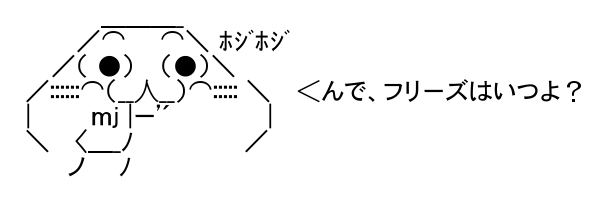
\includegraphics[width=1.1\hsize]{image201111/yaruo-freeze.png}
\end{center}
\end{frame}


\begin{frame}
\begin{center}
\LARGE{2012 年 6 月にフリーズ予定!}\\\pause

\LARGE{入れたいパッケージ、アップデートされてないパッケージがあったらそのへんのDebian関係者
を捕まえて言ってください。}
\end{center}
\end{frame}

\begin{frame}{リリースに向けてのご協力を!}
\begin{itemize}
 \item Debian を使ってください。
 \item squeezeにアップデートしましょう。
 \item バグ報告してください。些細なことでもなんでもOK。\\
2ch とか ブログに書くのは勘弁してください.....。\\
(トラッキングが難しいです)
 \item ドキュメント作成、翻訳に参加してください。\\
翻訳からTypoの指摘歓迎!
 \item パッケージメンテナンス等に興味がある方はサポートします。\\
そのへんにいる Debian 関係者に声をかけてください。
\end{itemize}
\end{frame}


\begin{frame}{質疑応答}
\begin{center}
\Large なにか質問はありますか?
\end{center}
\end{frame}

\begin{frame}{今後のイベント}
\begin{itemize}
\item 12月 東京エリア Debian勉強会 12月17日\\
場所: スクエア・エニックスさん
\item 12月 関西エリア Debian勉強会 {\color{red}クリスマス}\\
場所: 未定
\end{itemize}
詳細は \url{http://tokyodebian.alioth.debian.org}を参照

\end{frame}


\end{document}

;;; Local Variables: ***
;;; outline-regexp: "\\([ 	]*\\\\\\(documentstyle\\|documentclass\\|emtext\\|section\\|begin{frame}\\)\\*?[ 	]*[[{]\\|[]+\\)" ***
;;; End: ***
